%% 30 minutes

\documentclass[pdftex]{beamer}
%\setbeameroption{show notes}
\usepackage[T1]{fontenc}
\usepackage[utf8x]{inputenc}
\usepackage{theme/beamerthemeALU}

\usepackage{amsmath}
%\usepackage{amssymb}
%\usepackage{mathtools}
\usepackage{cmll} % \with

\usepackage{stmaryrd}
\usepackage{listings}
\usepackage{mathpartir}
\usepackage{pgf}
\usepackage{tikz}
\usetikzlibrary{arrows,automata}

\setbeamertemplate{navigation symbols}{}

\newcommand\code[2][]{\mbox{\lstinline[#1,basicstyle=\ttfamily\normalsize]{#2}}}
% Colors!
\definecolor{butter}{HTML}{C4A000}
\definecolor{orange}{HTML}{CE5C00}
\definecolor{chocolate}{HTML}{8F5902}
\definecolor{chameleon}{HTML}{4E9A06}
\definecolor{skyblue}{HTML}{204A87}
\definecolor{plum}{HTML}{5C3566}
\definecolor{scarletred}{HTML}{A40000}
\definecolor{lightalu}{HTML}{BABDB6}
\definecolor{darkalu}{HTML}{2E3436}
\newcommand{\kwstyle}{}

\lstdefinelanguage{Haskell}{
  otherkeywords={|,=>,<=,<,>,<>,::,=,@,||,\$},%
  keywords=[1]{if,then,else,case,of,in,let,where,do},
  keywords=[2]{class,data,newtype,deriving,type},%
  keywords=[3]{hiding,infix,infixl,infixr,import,instance,module,qualified},%
  keywordstyle=\kwstyle,
  keywordstyle=[1]\kwstyle\color{chameleon},
  keywordstyle=[2]\kwstyle\color{scarletred},
  keywordstyle=[3]\kwstyle\color{skyblue},
  keywordstyle=[4]\kwstyle\color{butter},
  keywordstyle=[5]\kwstyle\color{skyblue},
  keywordstyle=[6]\kwstyle\color{skyblue},
  keywordstyle=[7]\kwstyle\color{chameleon},
  keywordstyle=[8]\kwstyle\color{butter},
  keywordstyle=[9]\kwstyle\color{butter},
  sensitive,%
  comment=[l]{--},%
  comment=[n]{\{-}{-\}},%
  string=[b]",%
  literate={->}{{{\kwstyle\color{chameleon}->}}}2
}%

%% Code listing
\lstset{
  tabsize=4,
  aboveskip={0.5\baselineskip},
  belowcaptionskip=0.5\baselineskip,
  columns=fixed,keepspaces,
  showstringspaces=false,
  extendedchars=true,
  breaklines=true,
  frame=none,
  basicstyle=\small\ttfamily, %\scriptsize\ttfamily
  keywordstyle=\bfseries,
  commentstyle=\itshape\color{gray},
  % identifierstyle=\color{blue!80!black},
  stringstyle=\color{purple!40!black},
  numbersep=5pt,
  numberstyle=\tiny\color{gray},
  escapeinside={(*@}{@*)},
  numbers=left,
  emphstyle=\color{green!60!black}\bfseries,
  emphstyle={[2]\color{blue!60!black}\bfseries},
  language=Haskell
}


%%% regular expressions
\newcommand\Rnull{\mathbf0}
\newcommand\Rempty{\mathbf1}
\newcommand\Runion[1]{#1 +}
\newcommand\Rconcat[1]{#1 \cdot}
\newcommand\Rstar[1]{#1^*}
\newcommand\Rintersect[1]{#1 \with}
\newcommand\Rcomplement{\texttt{\textasciitilde}}

\newcommand\Lang[1]{\llbracket#1\rrbracket}

%%% misc
\newcommand\ltext[1]{\makebox[0pt][r]{\text{#1}\quad}}
\newcommand\lleq{\le_{ll}}

\newcommand\FPS[2][\Sigma]{#2\langle\!\langle#1^*\rangle\!\rangle}


\begin{document}
\everymath{\displaystyle}

% to enable title graphic enable this line, make sure the height is not too big
\titlegraphic{
\includegraphics[height=6em]{theme/Uni_Logo-Grundversion_E1_A4_CMYK}}

\title{Test Generation for Regular Expression Engines}
\author[Thiemann]%
{Gabriel Radanne and Peter Thiemann}
\institute[IIF]{University of Freiburg, Germany\\[4pt]
\texttt{thiemann@informatik.uni-freiburg.de}
}
%\date[\today]{\today}
\date[2018-05-02]{02 May 2018}

% begin titlepage
% "`normal"' front page template:
% \setbeamertemplate{title page}[default][rounded=true]
\makeatletter
\begin{frame}[plain,label=fp]
    \advance\textwidth by 3.2em\relax
    \begin{minipage}{\textwidth}\par%
      \maketitle
    \end{minipage}
    \hspace*{2.5em}%
\end{frame}
\makeatother 

\section{Prelude}
\AtBeginSection[]
{
 \begin{frame}<beamer>
 \frametitle{Plan}
 \tableofcontents[currentsection]
 \end{frame}
}

\begin{frame}
    \begin{center}
      
\includegraphics[scale=0.8]{regular-expressions-regex-everywhere}
    \end{center}
\end{frame}

\begin{frame}
  \frametitle{Regular expressions seem to be kind of important \dots}
  \begin{center}
    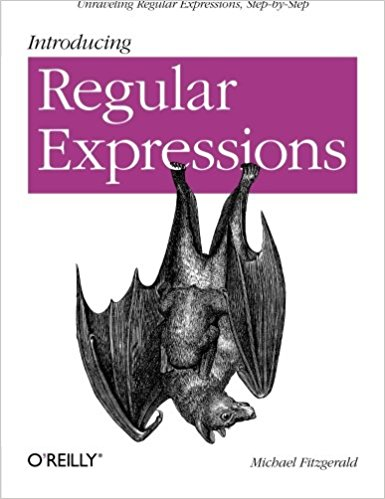
\includegraphics[scale=0.25]{book-introducing-regular-expressions}
    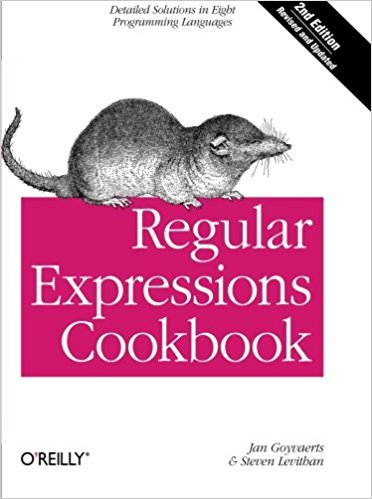
\includegraphics[scale=0.25]{book-regular-expression-cookbook}
    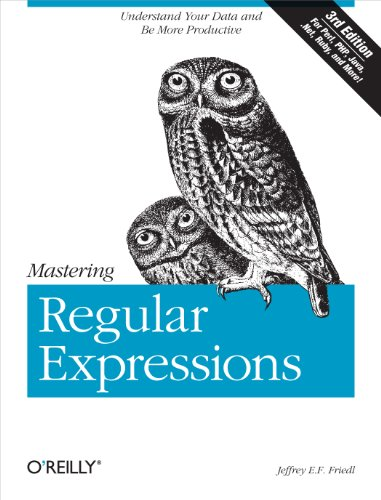
\includegraphics[scale=0.25]{book-mastering-regular-expressions}
  \end{center}
\end{frame}

\begin{frame}
  \frametitle{Uses abound}
  \begin{block}{Wikipedia sayz}
    Regexes are useful in a wide variety of text processing tasks, and
    more generally string processing, where the data need not be
    textual. Common applications include data validation, data
    scraping (especially web scraping), data wrangling, simple
    parsing, the production of syntax highlighting systems, and many
    other tasks.

    \url{https://en.wikipedia.org/wiki/Regular_expression\#Uses}
  \end{block}
\end{frame}

\begin{frame}
  \frametitle{Lots of Implementations}
  \begin{itemize}
  \item Many libraries
  \item Many programming languages
  \item Still new implementations and algorithms
  \end{itemize}
\end{frame}

\begin{frame}
  \frametitle{Motivation}
  \begin{block}<+->{Question}
    How do we test a regex implementation?
  \end{block}
  \begin{exampleblock}<+->{Answer}
    Create test cases.
  \end{exampleblock}
  \begin{block}<+->{Question}
    But the language of a regex can be infinite! How can we increase confidence?
  \end{block}
  \begin{exampleblock}<+->{Answer}
    Use random testing and employ any of the existing engines as an oracle!
  \end{exampleblock}
\end{frame}

\begin{frame}
  \frametitle{Motivation (cont'd)}
  \begin{block}<+->{Question}
    But how do I generate random test inputs fairly?
  \end{block}
  \begin{exampleblock}<+->{Answer}
    Huh?
  \end{exampleblock}
  \begin{block}<+->{Question}
    Consider the alphabet $\{a,b\}$ and the expression $a^*$. What is
    the probability that a randomly generated string is in $L (a^*)$?
  \end{block}
\end{frame}
\begin{frame}
  \frametitle{Motivation (cont'd)}
  \begin{exampleblock}<+->{Answer}
    \begin{displaymath}
      \lim_{n\to\infty} P (w \in L(a^*) \mid w \in \{a,b\}^{\le n})
    \end{displaymath}
  \end{exampleblock}
  \begin{block}<+->{Question}
    Aha?
  \end{block}
  \begin{exampleblock}<+->{Answer}
    \vspace{-\baselineskip}
    \begin{align*}
      \dots&= \lim_{n\to\infty} \frac{n+1}{\sum_{i=0}^n 2^i } &
      &= \lim_{n\to\infty} \frac{n+1}{ 2^{n+1} -1 }  &
      &=0
    \end{align*}
  \end{exampleblock}
\end{frame}
\begin{frame}
  \frametitle{Our Work}
  \begin{block}<+->{Given a regular expression $r$ generate}
    \begin{itemize}
    \item strings that are \textbf{definitely in} $L(r)$ and
    \item strings that are \textbf{definitely not in} $L(r)$
    \end{itemize}
  \end{block}
  \begin{block}<+->{Advantages}
    \begin{itemize}
    \item Positive and negative examples guaranteed 
    \item No oracle needed
    \item Exhaustive testing for (many) finite languages
    \end{itemize}
  \end{block}
\end{frame}
\begin{frame}
  \frametitle{Approach}
  \framesubtitle{What we actually do}
  \begin{Huge}
    \begin{center}
      \bf
      Language Generators for Extended Regular Expressions
    \end{center}
  \end{Huge}
\end{frame}
\begin{frame}
  \frametitle{Extended Regular Expressions}
  \vspace{-\baselineskip}
  \footnotesize
  \begin{align*}
    r, s & &\Lang{\_}=\quad &  &
                             \makebox[1em][l]{\code{data GRE sig}}\\
         & ::= \Rnull & \ltext{empty}
                        & \emptyset
                           &&\code{= Zero}\\
         & \mid \Rempty & \ltext{empty word}
                        & \{ \varepsilon \}
                           && \code{| One}\\
         & \mid (a \in \Sigma) & \ltext{singleton}
                        &  \{ a \}
                           && \code{| Atom sig} \\
         & \mid \Runion rs & \ltext{alternative}
                        &  \Lang{r} \cup \Lang{s}
                           && \code{| Or (GRE sig) (GRE sig)}\\
         & \mid \Rconcat rs & \ltext{concat}
                        &  \Lang r \cdot \Lang s
                           && \code{| Dot (GRE sig) (GRE sig)}\\
         & \mid \Rstar r & \ltext{closure}
                        & \Lang r^* 
                           && \code{| Star (GRE sig)}\\
         & \mid \Rintersect rs & \ltext{intersection}
                        & \Lang r \cap \Lang s
                           && \code{| And (GRE sig) (GRE sig)}\\
         & \mid \Rcomplement r & \ltext{complement}
                        & \Sigma^* \setminus \Lang r
                           && \code{| Not (GRE sig)}
  \end{align*}
\end{frame} 
\begin{frame}[fragile]
  \frametitle{Requirements}
  \begin{block}{Specification}
\begin{lstlisting}[numbers=none]
import Data.Text as T

type Alphabet = [Char]
type Lang = [T.Text]

generate :: Alphabet -> GRE Char -> Lang
\end{lstlisting}
  \end{block}
  \begin{itemize}
  \item No repetitions in output \code{Lang}.
  \item Output must not be partial / definition should be productive.
  \item Should be possible to throttle output with respect to word length.
  \item Generation should be compositional.
  \end{itemize}
\end{frame}
\begin{frame}[fragile]
  \frametitle{Compositional Spec}
\begin{lstlisting}[numbers=none]
generate :: Alphabet -> GRE Char -> Lang
generate sigma r = gen r
  where
    gen Zero = []
    gen One  = [T.empty]
    gen (Atom t) = [T.singleton t]
    gen (Or r s) = union (gen r) (gen s)
    gen (Dot r s) = concatenate (gen r) (gen s)
    gen (Star r) = star (gen r)
    gen (And r s) = intersect (gen r) (gen s)
    gen (Not r) = complement sigma (gen r)
\end{lstlisting}
\end{frame}
\begin{frame}[fragile]
  \frametitle{Naive Implementation}
\vspace{-2\baselineskip}
\begin{lstlisting}[numbers=none]
union :: Lang -> Lang -> Lang
union lx ly = lx ++ ly

concatenate :: Lang -> Lang -> Lang
concatenate lx ly =
  [T.append wx wy | wx <- lx, wy <- ly ]

intersect :: Lang -> Lang -> Lang
intersect lx ly = [wx | wx <- lx, wx `elem` ly ]

star :: Lang -> Lang
star lx = concat lxi
  where
    lxi = [T.empty] : map (concatenate lx) lxi

complement :: Alphabet -> Lang -> Lang
complement sigma lx =
  undefined
\end{lstlisting}
\end{frame}

\begin{frame}
  \frametitle{Lots of Problems}
  \begin{description}
  \item[duplicates] created by \code{union}, \code{concatenate}, and \code{star}.

    Could be addressed by \code{List.union} and \code{List.nub}.
  \item[unfairness] (union) If \texttt{lx} is infinite, then no words
    from \texttt{ly} will ever be produced.
    (concatenate) If \texttt{ly} is infinite, then only one word
    from \texttt{lx} will ever be considered.
  \item[partiality] Intersection may not produce a next element if \texttt{ly} is infinite.
  \end{description}
  \begin{block}<2->{Could be addressed \dots} by restricting to finite
    (subset of) languages.
    \begin{itemize}
    \item Unsatisfactory.
    \item Inefficient because of
    quadratic behavior of \code{List.union} and \code{List.nub}.
  \end{itemize}
  \end{block}
\end{frame}

\begin{frame}
  \frametitle{Questions}
  \begin{itemize}
  \item Can we do better?
  \item Can we support finite and infinite languages?
  \item Can we avoid extraneous quadratic behavior?
  \end{itemize}
\end{frame}
\begin{frame}[fragile]
  \frametitle{Ordered Enumeration}
  \vspace{-\baselineskip}
  \begin{block}<+->{Approach}
    \begin{itemize}
    \item Generate words in strictly ascending order
    \item Use length-lexicographic order to guarantee progress
    \item Cf.\ M. Douglas McIlroy:
      Enumerating the strings of regular languages. J. Funct. Program. 14(5): 503-518 (2004)
    \end{itemize}
  \end{block}
  \begin{block}<+->{Length-Lexicographic Order}
\begin{lstlisting}[numbers=none]
llocompare :: T.Text -> T.Text -> Ordering
llocompare u v =
  case compare (T.length u) (T.length v) of
    EQ -> compare u v
    LT -> LT
    GT -> GT
\end{lstlisting}
  \end{block}
\end{frame}
\begin{frame}[fragile,fragile]
  \frametitle{Union, Intersection, and Difference by Merging}
\begin{lstlisting}[numbers=none]
union :: Lang -> Lang -> Lang
union xs@(x:xt) ys@(y:yt) =
  case llocompare x y of
    EQ -> x : union xt yt
    LT -> x : union xt ys
    GT -> y : union xs yt
union xs ys = xs ++ ys
\end{lstlisting}
  \begin{itemize}
  \item intersection and difference are analogous
  \item productive, linear time
  \end{itemize}
\end{frame}

\begin{frame}[fragile]
  \frametitle{Concatenation a la McIlroy}
\begin{lstlisting}[numbers=none]
concatenate :: Lang -> Lang -> Lang
concatenate [] ly = []
concatenate lx [] = []
concatenate (x:xt) ly@(y:yt) =
  T.append x y : union (concatenate [x] yt) 
                       (concatenate xt ly)
\end{lstlisting}
\end{frame}

\begin{frame}[fragile,fragile]
  \frametitle{Closure a la McIlroy }
\begin{lstlisting}[numbers=none]
star :: Lang -> Lang
star [] = [T.empty]
star lx@(x:xt)
  | x == T.empty = star xt
  | otherwise =
    T.empty : concatenate lx (star lx)
\end{lstlisting}
\end{frame}

\begin{frame}[fragile]
  \frametitle{Complement}
\begin{lstlisting}[numbers=none]
complement :: Alphabet -> Lang -> Lang
complement sigma lx = difference lsigmastar lx
  where
    lsigmastar = star (map T.singleton sigma)
\end{lstlisting}
\end{frame}

\begin{frame}[fragile]
  \frametitle{What did we achieve so far?}
  \begin{itemize}
  \item<+-> efficient definitions for all operations needed in extended regular expressions
  \item<+-> productive definitions for for \code{union},
    \code{intersection}, \code{concatenate}, \code{star}
  \end{itemize}
  \begin{block}<+->{But}
    \begin{itemize}
    \item partial results for some expressions involving complement
    \item cannot throttle with a length bound
  \end{itemize}
  \end{block}
  \begin{exampleblock}<+->{Partial, nonterminating example}
\begin{lstlisting}[numbers=none]
complement "ab" (star (map T.singleton "ab"))
\end{lstlisting}
  \end{exampleblock}
\end{frame}
\begin{frame}
  \frametitle{Towards a Different Representation for Languages}
  \vspace{-\baselineskip}
  \begin{block}<+->{Inspiration: Formal Power Series}
    Represent language by a power series    where, for all $n$, $L_n \subseteq \Sigma^n$.
    \begin{gather*}
      L = \sum_{n=0}^\infty L_nx^n
    \end{gather*}
  \end{block}
  \begin{block}<+->{Facts}
    \begin{itemize}
    \item Each $L_n$ is a \textbf{finite language}.
    \item Can choose an efficient representation for the $L_n$.
    \end{itemize}
  \end{block}
\end{frame}
\begin{frame}
  \frametitle{Operations on Power Series}
\begin{block}<+->{Operations}
  \vspace{-\baselineskip}
    \begin{align*}
      L \cup M & = \sum_{n=0}^\infty (L_n \cup M_n)x^n & \text{union}\\
      L \cap M & = \sum_{n=0}^\infty (L_n \cap M_n)x^n & \text{Hadamard product} \\
      L \cdot M &= \sum_{n=0}^\infty (\bigcup_{i=0}^n L_i \cdot M_{n-i})x^n & \text{product}
    \end{align*}
  \end{block}
\end{frame}
\begin{frame}
  \frametitle{More Operations}
  \begin{block}{Star Operation}
    \vspace{-\baselineskip}
    \begin{align*}
      L^* &= \sum_{n=0}^\infty R_n x^n
      \intertext{where}
      R_0 &= \{ \varepsilon \} \\
      R_{i+1} &= L_{i+1} \cup L_i \cdot R_1 \cup \dots \cup L_1 \cdot R_i\\
      &= \bigcup_{j=0}^i L_{j+1} \cdot R_{i-j}
    \end{align*}
    a proper inductive definition!
  \end{block}
\end{frame}
\begin{frame}
  \frametitle{Data Structures}
  \begin{block}<+->{\dots{} for $L_n$ (segments)}
    \begin{itemize}
    \item \code{[T.Text]} with standard ordering and operations defined by merge
    \item \code{Data.Set.Set T.Text} with its operations
    \item other choices, e.g., tries
    \end{itemize}
  \end{block}
  \begin{block}<+->{\dots{} for implementing the operations}
    \begin{itemize}
    \item input and output are lazy streams of segments $[L_0, L_1, L_2, \dots]$
    \end{itemize}
  \end{block}
\end{frame}
\begin{frame}[fragile]
  \frametitle{Incremental Computation}
  \framesubtitle{Product}
  \vspace{-2\baselineskip}
  \begin{align*}
    (L \cdot M)_n & = \bigcup_{i=0}^n L_i \cdot M_{n-i}
  \end{align*}
  \begin{align*}
    \code{lx} &= [L_0, L_1, L_2, \dots ] & \text{given}\\
    \code{mxrev} &= [M_n, M_{n-1}, \dots , M_0] & \text{compute incrementally}
  \end{align*}
  \begin{block}<2->{Implementation}
\begin{lstlisting}[numbers=none]
concatenate lx mx = collect mx []
  where -- hidden lemma
    collect (mxh:mx') mxrev =
      let mxrev' = mxh:mxrev in
        foldr S.union S.empty
        (zipWith T.append lx mxrev') :
        collect mx' mxrev'
\end{lstlisting}
  \end{block}
\end{frame}
\begin{frame}[fragile]
  \frametitle{Incremental Computation}
  \framesubtitle{Closure}
  \vspace{-2\baselineskip}
  \begin{align*}
    (L^*)_0 & = \{\varepsilon\} \\
    (L^*)_{n+1} & = \bigcup_{i=0}^n L_{i+1} \cdot (L^*)_{n-i}
                  &&= \bigcup_{i=0}^n L_{n+1-i} \cdot (L^*)_i
  \end{align*}
  \begin{block}{Implementation}
\begin{lstlisting}[numbers=none]
star lx = slx
  where
    slx = S.singleton (T.empty) :
          collect (tail lx) []
    collect (lxh:lx') lxrev =
      let lxrev' = lxh:lxrev in
        foldr S.union S.empty
        (zipWith T.append lxrev' slx) :
        collect lx' lxrev'
\end{lstlisting}
  \end{block}
\end{frame}
\begin{frame}
  \frametitle{Improvements}
  \begin{block}{Language representation}
  \begin{itemize}
  \item Finite list of segments if all further segments are empty
  \item Finite list of segments if all further segments are full
  \item[$\Rightarrow$] Recognize (many) finite and cofinite languages
  \item Can be maintained through all operations except Kleene closure
  \end{itemize}
\end{block}
\end{frame}
\begin{frame}
  \frametitle{Benchmarks}
    \begin{itemize}
    \item Implementations in Haskell and OCaml
    \end{itemize}
\end{frame}
\begin{frame}
  \frametitle{Conclusions}
  \begin{block}<+->{Good basis for language generator}
    \begin{itemize}
    \item Efficient and productive definitions for all operations
    \item No partiality
    \item Throttling with length bound straightforward
    \end{itemize}
  \end{block}
  \begin{block}<+->{Extensible to other language generators}
    \begin{itemize}
    \item finite automata
    \item context-free grammars
    \item conjunctive grammars
    \item any decidable language representable as a stream of segments \dots
    \end{itemize}
  \end{block}
\end{frame}
\end{document}
%%% Local Variables: 
%%% mode: latex
%%% TeX-master: t
%%% End: 
